\documentclass[twoside]{book}

% Packages required by doxygen
\usepackage{calc}
\usepackage{doxygen}
\usepackage{graphicx}
\usepackage[utf8]{inputenc}
\usepackage{makeidx}
\usepackage{multicol}
\usepackage{multirow}
\usepackage{textcomp}
\usepackage[table]{xcolor}

% Font selection
\usepackage[T1]{fontenc}
\usepackage{mathptmx}
\usepackage[scaled=.90]{helvet}
\usepackage{courier}
\usepackage{amssymb}
\usepackage{sectsty}
\renewcommand{\familydefault}{\sfdefault}
\allsectionsfont{%
  \fontseries{bc}\selectfont%
  \color{darkgray}%
}
\renewcommand{\DoxyLabelFont}{%
  \fontseries{bc}\selectfont%
  \color{darkgray}%
}

% Page & text layout
\usepackage{geometry}
\geometry{%
  a4paper,%
  top=2.5cm,%
  bottom=2.5cm,%
  left=2.5cm,%
  right=2.5cm%
}
\tolerance=750
\hfuzz=15pt
\hbadness=750
\setlength{\emergencystretch}{15pt}
\setlength{\parindent}{0cm}
\setlength{\parskip}{0.2cm}
\makeatletter
\renewcommand{\paragraph}{%
  \@startsection{paragraph}{4}{0ex}{-1.0ex}{1.0ex}{%
    \normalfont\normalsize\bfseries\SS@parafont%
  }%
}
\renewcommand{\subparagraph}{%
  \@startsection{subparagraph}{5}{0ex}{-1.0ex}{1.0ex}{%
    \normalfont\normalsize\bfseries\SS@subparafont%
  }%
}
\makeatother

% Headers & footers
\usepackage{fancyhdr}
\pagestyle{fancyplain}
\fancyhead[LE]{\fancyplain{}{\bfseries\thepage}}
\fancyhead[CE]{\fancyplain{}{}}
\fancyhead[RE]{\fancyplain{}{\bfseries\leftmark}}
\fancyhead[LO]{\fancyplain{}{\bfseries\rightmark}}
\fancyhead[CO]{\fancyplain{}{}}
\fancyhead[RO]{\fancyplain{}{\bfseries\thepage}}
\fancyfoot[LE]{\fancyplain{}{}}
\fancyfoot[CE]{\fancyplain{}{}}
\fancyfoot[RE]{\fancyplain{}{\bfseries\scriptsize Generated on Tue Mar 18 2014 13\-:24\-:43 for T\-H\-O3 Kevin Nijmijer, Peter Markotiç, Michiel Tegelberg by Doxygen }}
\fancyfoot[LO]{\fancyplain{}{\bfseries\scriptsize Generated on Tue Mar 18 2014 13\-:24\-:43 for T\-H\-O3 Kevin Nijmijer, Peter Markotiç, Michiel Tegelberg by Doxygen }}
\fancyfoot[CO]{\fancyplain{}{}}
\fancyfoot[RO]{\fancyplain{}{}}
\renewcommand{\footrulewidth}{0.4pt}
\renewcommand{\chaptermark}[1]{%
  \markboth{#1}{}%
}
\renewcommand{\sectionmark}[1]{%
  \markright{\thesection\ #1}%
}

% Indices & bibliography
\usepackage{natbib}
\usepackage[titles]{tocloft}
\setcounter{tocdepth}{3}
\setcounter{secnumdepth}{5}
\makeindex

% Hyperlinks (required, but should be loaded last)
\usepackage{ifpdf}
\ifpdf
  \usepackage[pdftex,pagebackref=true]{hyperref}
\else
  \usepackage[ps2pdf,pagebackref=true]{hyperref}
\fi
\hypersetup{%
  colorlinks=true,%
  linkcolor=blue,%
  citecolor=blue,%
  unicode%
}

% Custom commands
\newcommand{\clearemptydoublepage}{%
  \newpage{\pagestyle{empty}\cleardoublepage}%
}


%===== C O N T E N T S =====

\begin{document}

% Titlepage & ToC
\hypersetup{pageanchor=false}
\pagenumbering{roman}
\begin{titlepage}
\vspace*{7cm}
\begin{center}%
{\Large T\-H\-O3 Kevin Nijmijer, Peter Markotiç, Michiel Tegelberg }\\
\vspace*{1cm}
{\large Generated by Doxygen 1.8.5}\\
\vspace*{0.5cm}
{\small Tue Mar 18 2014 13:24:43}\\
\end{center}
\end{titlepage}
\clearemptydoublepage
\tableofcontents
\clearemptydoublepage
\pagenumbering{arabic}
\hypersetup{pageanchor=true}

%--- Begin generated contents ---
\chapter{Hierarchical Index}
\section{Class Hierarchy}
This inheritance list is sorted roughly, but not completely, alphabetically\-:\begin{DoxyCompactList}
\item \contentsline{section}{Calibrate}{\pageref{class_calibrate}}{}
\item Color\-Sensor\begin{DoxyCompactList}
\item \contentsline{section}{My\-Color\-Sensor}{\pageref{class_my_color_sensor}}{}
\end{DoxyCompactList}
\item \contentsline{section}{Drive\-Controller}{\pageref{class_drive_controller}}{}
\item \contentsline{section}{Main}{\pageref{class_main}}{}
\item \contentsline{section}{Robot\-Controller}{\pageref{class_robot_controller}}{}
\item \contentsline{section}{Sensor\-Listener}{\pageref{interface_sensor_listener}}{}
\begin{DoxyCompactList}
\item \contentsline{section}{Sensor\-Controller}{\pageref{class_sensor_controller}}{}
\end{DoxyCompactList}
\item Thread\begin{DoxyCompactList}
\item \contentsline{section}{Sensor\-Handler}{\pageref{class_sensor_handler}}{}
\end{DoxyCompactList}
\item Ultrasonic\-Sensor\begin{DoxyCompactList}
\item \contentsline{section}{My\-Ultrasonic\-Sensor}{\pageref{class_my_ultrasonic_sensor}}{}
\end{DoxyCompactList}
\item \contentsline{section}{Updating\-Sensor}{\pageref{interface_updating_sensor}}{}
\begin{DoxyCompactList}
\item \contentsline{section}{My\-Color\-Sensor}{\pageref{class_my_color_sensor}}{}
\item \contentsline{section}{My\-Ultrasonic\-Sensor}{\pageref{class_my_ultrasonic_sensor}}{}
\end{DoxyCompactList}
\end{DoxyCompactList}

\chapter{Class Index}
\section{Class List}
Here are the classes, structs, unions and interfaces with brief descriptions\-:\begin{DoxyCompactList}
\item\contentsline{section}{\hyperlink{class_calibrate}{Calibrate} }{\pageref{class_calibrate}}{}
\item\contentsline{section}{\hyperlink{class_drive_controller}{Drive\-Controller} }{\pageref{class_drive_controller}}{}
\item\contentsline{section}{\hyperlink{class_main}{Main} }{\pageref{class_main}}{}
\item\contentsline{section}{\hyperlink{class_my_color_sensor}{My\-Color\-Sensor} }{\pageref{class_my_color_sensor}}{}
\item\contentsline{section}{\hyperlink{class_my_ultrasonic_sensor}{My\-Ultrasonic\-Sensor} }{\pageref{class_my_ultrasonic_sensor}}{}
\item\contentsline{section}{\hyperlink{class_robot_controller}{Robot\-Controller} }{\pageref{class_robot_controller}}{}
\item\contentsline{section}{\hyperlink{class_sensor_controller}{Sensor\-Controller} }{\pageref{class_sensor_controller}}{}
\item\contentsline{section}{\hyperlink{class_sensor_handler}{Sensor\-Handler} }{\pageref{class_sensor_handler}}{}
\item\contentsline{section}{\hyperlink{interface_sensor_listener}{Sensor\-Listener} }{\pageref{interface_sensor_listener}}{}
\item\contentsline{section}{\hyperlink{interface_updating_sensor}{Updating\-Sensor} }{\pageref{interface_updating_sensor}}{}
\end{DoxyCompactList}

\chapter{Class Documentation}
\hypertarget{class_calibrate}{\section{Calibrate Class Reference}
\label{class_calibrate}\index{Calibrate@{Calibrate}}
}
\subsection*{Public Member Functions}
\begin{DoxyCompactItemize}
\item 
\hyperlink{class_calibrate_a2c63215e4b4a27142f941900b9cdd8f1}{Calibrate} ()
\item 
void \hyperlink{class_calibrate_a5d0acb6ebc5410f9c720e4cd747f30d8}{calibrate\-Senors} ()
\item 
\hyperlink{class_my_color_sensor}{My\-Color\-Sensor} \hyperlink{class_calibrate_ae94a70d48193edadb902e1886f7f8f02}{get\-Right} ()
\item 
\hyperlink{class_my_color_sensor}{My\-Color\-Sensor} \hyperlink{class_calibrate_a7770009a94d2de4c31f472c3ddd3c53c}{get\-Left} ()
\end{DoxyCompactItemize}


\subsection{Detailed Description}
\begin{DoxyAuthor}{Author}
Peter Markoti�, Kevin Nijmijer, Michiel Tegelberg 
\end{DoxyAuthor}
\begin{DoxyVersion}{Version}
1.\-0 
\end{DoxyVersion}


\subsection{Constructor \& Destructor Documentation}
\hypertarget{class_calibrate_a2c63215e4b4a27142f941900b9cdd8f1}{\index{Calibrate@{Calibrate}!Calibrate@{Calibrate}}
\index{Calibrate@{Calibrate}!Calibrate@{Calibrate}}
\subsubsection[{Calibrate}]{\setlength{\rightskip}{0pt plus 5cm}Calibrate.\-Calibrate (
\begin{DoxyParamCaption}
{}
\end{DoxyParamCaption}
)}}\label{class_calibrate_a2c63215e4b4a27142f941900b9cdd8f1}
Constructor for the \hyperlink{class_calibrate}{Calibrate} class. Makes instances of \hyperlink{class_my_color_sensor}{My\-Color\-Sensor} for the right and left Color\-Sensor. Sets the floodlights for the left and right Color\-Sensor. 

\subsection{Member Function Documentation}
\hypertarget{class_calibrate_a5d0acb6ebc5410f9c720e4cd747f30d8}{\index{Calibrate@{Calibrate}!calibrate\-Senors@{calibrate\-Senors}}
\index{calibrate\-Senors@{calibrate\-Senors}!Calibrate@{Calibrate}}
\subsubsection[{calibrate\-Senors}]{\setlength{\rightskip}{0pt plus 5cm}void Calibrate.\-calibrate\-Senors (
\begin{DoxyParamCaption}
{}
\end{DoxyParamCaption}
)}}\label{class_calibrate_a5d0acb6ebc5410f9c720e4cd747f30d8}
Function to aid the user with calibrating the sensors Takes the user through the process of calibrating all Color\-Sensors.

\begin{DoxyReturn}{Returns}
void 
\end{DoxyReturn}
\hypertarget{class_calibrate_a7770009a94d2de4c31f472c3ddd3c53c}{\index{Calibrate@{Calibrate}!get\-Left@{get\-Left}}
\index{get\-Left@{get\-Left}!Calibrate@{Calibrate}}
\subsubsection[{get\-Left}]{\setlength{\rightskip}{0pt plus 5cm}{\bf My\-Color\-Sensor} Calibrate.\-get\-Left (
\begin{DoxyParamCaption}
{}
\end{DoxyParamCaption}
)}}\label{class_calibrate_a7770009a94d2de4c31f472c3ddd3c53c}
Function to get the left calibrated \hyperlink{class_my_color_sensor}{My\-Color\-Sensor}.

\begin{DoxyReturn}{Returns}
\hyperlink{class_my_color_sensor}{My\-Color\-Sensor} left\-Eye 
\end{DoxyReturn}
\hypertarget{class_calibrate_ae94a70d48193edadb902e1886f7f8f02}{\index{Calibrate@{Calibrate}!get\-Right@{get\-Right}}
\index{get\-Right@{get\-Right}!Calibrate@{Calibrate}}
\subsubsection[{get\-Right}]{\setlength{\rightskip}{0pt plus 5cm}{\bf My\-Color\-Sensor} Calibrate.\-get\-Right (
\begin{DoxyParamCaption}
{}
\end{DoxyParamCaption}
)}}\label{class_calibrate_ae94a70d48193edadb902e1886f7f8f02}
Function to get the right calibrated \hyperlink{class_my_color_sensor}{My\-Color\-Sensor}.

\begin{DoxyReturn}{Returns}
\hyperlink{class_my_color_sensor}{My\-Color\-Sensor} right\-Eye 
\end{DoxyReturn}


The documentation for this class was generated from the following file\-:\begin{DoxyCompactItemize}
\item 
Calibrate.\-java\end{DoxyCompactItemize}

\hypertarget{class_drive_controller}{\section{Drive\-Controller Class Reference}
\label{class_drive_controller}\index{Drive\-Controller@{Drive\-Controller}}
}
\subsection*{Public Member Functions}
\begin{DoxyCompactItemize}
\item 
\hyperlink{class_drive_controller_a60cc3007214f3b790301fe0f38f31258}{Drive\-Controller} ()
\item 
void \hyperlink{class_drive_controller_af219e8f28401307c2f48b3f84076cd32}{drive} (int v)
\item 
void \hyperlink{class_drive_controller_af2f91d13c56233955273a599969ba85d}{stop} ()
\item 
void \hyperlink{class_drive_controller_a31cbe81465f7134c2fa868a00f01c6fb}{reset\-Tacho\-Counts} ()
\item 
int \hyperlink{class_drive_controller_a07150350921a814306f66c82ef633e3f}{get\-Tacho\-A} ()
\item 
int \hyperlink{class_drive_controller_aff45070da8524060767daceff546d85e}{get\-Tacho\-C} ()
\item 
void \hyperlink{class_drive_controller_a48cee304bd9808b851a0e2a7695dd00b}{correct\-Right} ()
\item 
void \hyperlink{class_drive_controller_a9d54a054f61fad504f637f1a63fdb907}{correct\-Left} ()
\item 
void \hyperlink{class_drive_controller_ac967935ad5712f94001ac298448fdf51}{evade} ()
\end{DoxyCompactItemize}


\subsection{Detailed Description}
\begin{DoxyAuthor}{Author}
Peter Markoti�, Kevin Nijmijer, Michiel Tegelberg 
\end{DoxyAuthor}
\begin{DoxyVersion}{Version}
2.\-0 
\end{DoxyVersion}


\subsection{Constructor \& Destructor Documentation}
\hypertarget{class_drive_controller_a60cc3007214f3b790301fe0f38f31258}{\index{Drive\-Controller@{Drive\-Controller}!Drive\-Controller@{Drive\-Controller}}
\index{Drive\-Controller@{Drive\-Controller}!DriveController@{Drive\-Controller}}
\subsubsection[{Drive\-Controller}]{\setlength{\rightskip}{0pt plus 5cm}Drive\-Controller.\-Drive\-Controller (
\begin{DoxyParamCaption}
{}
\end{DoxyParamCaption}
)}}\label{class_drive_controller_a60cc3007214f3b790301fe0f38f31258}
Constructor for the Motor\-Controller Calls N\-X\-T motor instances. 

\subsection{Member Function Documentation}
\hypertarget{class_drive_controller_a9d54a054f61fad504f637f1a63fdb907}{\index{Drive\-Controller@{Drive\-Controller}!correct\-Left@{correct\-Left}}
\index{correct\-Left@{correct\-Left}!DriveController@{Drive\-Controller}}
\subsubsection[{correct\-Left}]{\setlength{\rightskip}{0pt plus 5cm}void Drive\-Controller.\-correct\-Left (
\begin{DoxyParamCaption}
{}
\end{DoxyParamCaption}
)}}\label{class_drive_controller_a9d54a054f61fad504f637f1a63fdb907}
Stops the right motor so the robot turns left.

\begin{DoxyReturn}{Returns}
void 
\end{DoxyReturn}
\hypertarget{class_drive_controller_a48cee304bd9808b851a0e2a7695dd00b}{\index{Drive\-Controller@{Drive\-Controller}!correct\-Right@{correct\-Right}}
\index{correct\-Right@{correct\-Right}!DriveController@{Drive\-Controller}}
\subsubsection[{correct\-Right}]{\setlength{\rightskip}{0pt plus 5cm}void Drive\-Controller.\-correct\-Right (
\begin{DoxyParamCaption}
{}
\end{DoxyParamCaption}
)}}\label{class_drive_controller_a48cee304bd9808b851a0e2a7695dd00b}
Stops the left motor so the robot turns right.

\begin{DoxyReturn}{Returns}
void 
\end{DoxyReturn}
\hypertarget{class_drive_controller_af219e8f28401307c2f48b3f84076cd32}{\index{Drive\-Controller@{Drive\-Controller}!drive@{drive}}
\index{drive@{drive}!DriveController@{Drive\-Controller}}
\subsubsection[{drive}]{\setlength{\rightskip}{0pt plus 5cm}void Drive\-Controller.\-drive (
\begin{DoxyParamCaption}
\item[{int}]{v}
\end{DoxyParamCaption}
)}}\label{class_drive_controller_af219e8f28401307c2f48b3f84076cd32}
Sets speed v and sets both motors to drive forward.


\begin{DoxyParams}{Parameters}
{\em v} & velocity of the robot \\
\hline
\end{DoxyParams}
\begin{DoxyReturn}{Returns}
void 
\end{DoxyReturn}
\hypertarget{class_drive_controller_ac967935ad5712f94001ac298448fdf51}{\index{Drive\-Controller@{Drive\-Controller}!evade@{evade}}
\index{evade@{evade}!DriveController@{Drive\-Controller}}
\subsubsection[{evade}]{\setlength{\rightskip}{0pt plus 5cm}void Drive\-Controller.\-evade (
\begin{DoxyParamCaption}
{}
\end{DoxyParamCaption}
)}}\label{class_drive_controller_ac967935ad5712f94001ac298448fdf51}
Initiates an evasive maneuver in which the robot attempts to drive around an obstacle in a clockwise arc.

\begin{DoxyReturn}{Returns}
void 
\end{DoxyReturn}
\hypertarget{class_drive_controller_a07150350921a814306f66c82ef633e3f}{\index{Drive\-Controller@{Drive\-Controller}!get\-Tacho\-A@{get\-Tacho\-A}}
\index{get\-Tacho\-A@{get\-Tacho\-A}!DriveController@{Drive\-Controller}}
\subsubsection[{get\-Tacho\-A}]{\setlength{\rightskip}{0pt plus 5cm}int Drive\-Controller.\-get\-Tacho\-A (
\begin{DoxyParamCaption}
{}
\end{DoxyParamCaption}
)}}\label{class_drive_controller_a07150350921a814306f66c82ef633e3f}
Returns the tacho\-Count for the left motor.

\begin{DoxyReturn}{Returns}
int 
\end{DoxyReturn}
\hypertarget{class_drive_controller_aff45070da8524060767daceff546d85e}{\index{Drive\-Controller@{Drive\-Controller}!get\-Tacho\-C@{get\-Tacho\-C}}
\index{get\-Tacho\-C@{get\-Tacho\-C}!DriveController@{Drive\-Controller}}
\subsubsection[{get\-Tacho\-C}]{\setlength{\rightskip}{0pt plus 5cm}int Drive\-Controller.\-get\-Tacho\-C (
\begin{DoxyParamCaption}
{}
\end{DoxyParamCaption}
)}}\label{class_drive_controller_aff45070da8524060767daceff546d85e}
Returns the tacho\-Count for the right motor.

\begin{DoxyReturn}{Returns}
int 
\end{DoxyReturn}
\hypertarget{class_drive_controller_a31cbe81465f7134c2fa868a00f01c6fb}{\index{Drive\-Controller@{Drive\-Controller}!reset\-Tacho\-Counts@{reset\-Tacho\-Counts}}
\index{reset\-Tacho\-Counts@{reset\-Tacho\-Counts}!DriveController@{Drive\-Controller}}
\subsubsection[{reset\-Tacho\-Counts}]{\setlength{\rightskip}{0pt plus 5cm}void Drive\-Controller.\-reset\-Tacho\-Counts (
\begin{DoxyParamCaption}
{}
\end{DoxyParamCaption}
)}}\label{class_drive_controller_a31cbe81465f7134c2fa868a00f01c6fb}
Resets the Tacho\-Count for both motors

\begin{DoxyReturn}{Returns}
void 
\end{DoxyReturn}
\hypertarget{class_drive_controller_af2f91d13c56233955273a599969ba85d}{\index{Drive\-Controller@{Drive\-Controller}!stop@{stop}}
\index{stop@{stop}!DriveController@{Drive\-Controller}}
\subsubsection[{stop}]{\setlength{\rightskip}{0pt plus 5cm}void Drive\-Controller.\-stop (
\begin{DoxyParamCaption}
{}
\end{DoxyParamCaption}
)}}\label{class_drive_controller_af2f91d13c56233955273a599969ba85d}
Stops the robot

\begin{DoxyReturn}{Returns}
void 
\end{DoxyReturn}


The documentation for this class was generated from the following file\-:\begin{DoxyCompactItemize}
\item 
Drive\-Controller.\-java\end{DoxyCompactItemize}

\hypertarget{class_main}{\section{Main Class Reference}
\label{class_main}\index{Main@{Main}}
}
\subsection*{Static Public Member Functions}
\begin{DoxyCompactItemize}
\item 
static void \hyperlink{class_main_a8a5d0f827edddff706cc0e6740d0579a}{main} (String\mbox{[}$\,$\mbox{]} args)
\end{DoxyCompactItemize}


\subsection{Member Function Documentation}
\hypertarget{class_main_a8a5d0f827edddff706cc0e6740d0579a}{\index{Main@{Main}!main@{main}}
\index{main@{main}!Main@{Main}}
\subsubsection[{main}]{\setlength{\rightskip}{0pt plus 5cm}static void Main.\-main (
\begin{DoxyParamCaption}
\item[{String\mbox{[}$\,$\mbox{]}}]{args}
\end{DoxyParamCaption}
)\hspace{0.3cm}{\ttfamily [static]}}}\label{class_main_a8a5d0f827edddff706cc0e6740d0579a}
\begin{DoxyAuthor}{Author}
Peter Markoti�, Kevin Nijmijer, Michiel Tegelberg 
\end{DoxyAuthor}
\begin{DoxyVersion}{Version}
3.\-0
\end{DoxyVersion}
The main thread starts by making a new instance of the \hyperlink{class_calibrate}{Calibrate} class. Then it calls Calibrate.\-calibrate\-Sensors() which prompts the user to go through the calibration process. After that the main thread makes an instance of \hyperlink{class_robot_controller}{Robot\-Controller} with the calibrated left and right My\-Color\-Sensors. Lastly the main calls \hyperlink{class_robot_controller_a81581974756705e965436ce7b9aff352}{Robot\-Controller.\-drive\-Robot()} which makes the robot drive autonomously. 

The documentation for this class was generated from the following file\-:\begin{DoxyCompactItemize}
\item 
Main.\-java\end{DoxyCompactItemize}

\hypertarget{class_my_color_sensor}{\section{My\-Color\-Sensor Class Reference}
\label{class_my_color_sensor}\index{My\-Color\-Sensor@{My\-Color\-Sensor}}
}
Inheritance diagram for My\-Color\-Sensor\-:\begin{figure}[H]
\begin{center}
\leavevmode
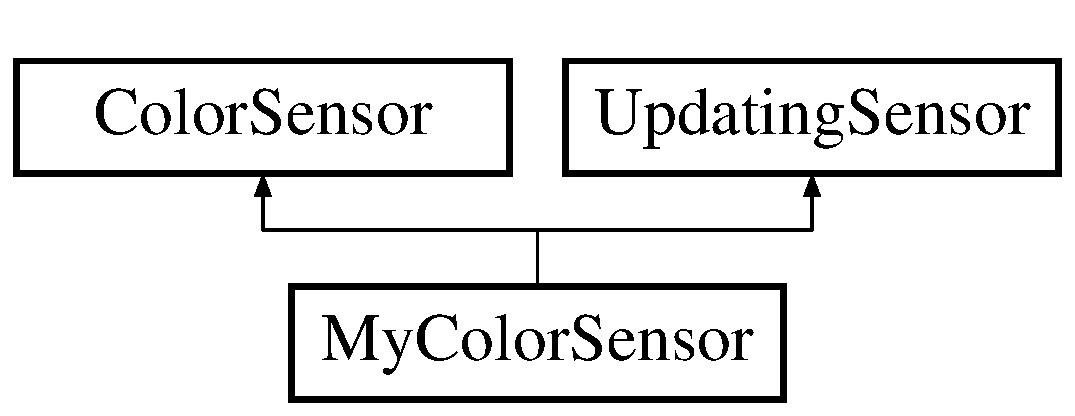
\includegraphics[height=2.000000cm]{class_my_color_sensor}
\end{center}
\end{figure}
\subsection*{Public Member Functions}
\begin{DoxyCompactItemize}
\item 
\hyperlink{class_my_color_sensor_a5716caf48342b95aeeb0dbc3ec3603b9}{My\-Color\-Sensor} (Sensor\-Port port, int s\-N)
\item 
void \hyperlink{class_my_color_sensor_ab5ffcfbfc721332303a0c5f3d341c541}{add\-Listener} (\hyperlink{interface_sensor_listener}{Sensor\-Listener} lst)
\item 
synchronized void \hyperlink{class_my_color_sensor_a4a839af511075bcfa34235513103d835}{update\-State} ()
\end{DoxyCompactItemize}


\subsection{Detailed Description}
\begin{DoxyAuthor}{Author}
Peter Markoti�, Kevin Nijmijer, Michiel Tegelberg 
\end{DoxyAuthor}
\begin{DoxyVersion}{Version}
2.\-0 
\end{DoxyVersion}


\subsection{Constructor \& Destructor Documentation}
\hypertarget{class_my_color_sensor_a5716caf48342b95aeeb0dbc3ec3603b9}{\index{My\-Color\-Sensor@{My\-Color\-Sensor}!My\-Color\-Sensor@{My\-Color\-Sensor}}
\index{My\-Color\-Sensor@{My\-Color\-Sensor}!MyColorSensor@{My\-Color\-Sensor}}
\subsubsection[{My\-Color\-Sensor}]{\setlength{\rightskip}{0pt plus 5cm}My\-Color\-Sensor.\-My\-Color\-Sensor (
\begin{DoxyParamCaption}
\item[{Sensor\-Port}]{port, }
\item[{int}]{s\-N}
\end{DoxyParamCaption}
)}}\label{class_my_color_sensor_a5716caf48342b95aeeb0dbc3ec3603b9}
Constructor for \hyperlink{class_my_color_sensor}{My\-Color\-Sensor}.


\begin{DoxyParams}{Parameters}
{\em port} & The port the sensor is connected to. \\
\hline
{\em s\-N} & The number of the sensor. \\
\hline
\end{DoxyParams}


\subsection{Member Function Documentation}
\hypertarget{class_my_color_sensor_ab5ffcfbfc721332303a0c5f3d341c541}{\index{My\-Color\-Sensor@{My\-Color\-Sensor}!add\-Listener@{add\-Listener}}
\index{add\-Listener@{add\-Listener}!MyColorSensor@{My\-Color\-Sensor}}
\subsubsection[{add\-Listener}]{\setlength{\rightskip}{0pt plus 5cm}void My\-Color\-Sensor.\-add\-Listener (
\begin{DoxyParamCaption}
\item[{{\bf Sensor\-Listener}}]{lst}
\end{DoxyParamCaption}
)}}\label{class_my_color_sensor_ab5ffcfbfc721332303a0c5f3d341c541}
Add a \hyperlink{interface_sensor_listener}{Sensor\-Listener} to pass values on to.


\begin{DoxyParams}{Parameters}
{\em lst} & The Listener \\
\hline
\end{DoxyParams}
\begin{DoxyReturn}{Returns}
void 
\end{DoxyReturn}
\hypertarget{class_my_color_sensor_a4a839af511075bcfa34235513103d835}{\index{My\-Color\-Sensor@{My\-Color\-Sensor}!update\-State@{update\-State}}
\index{update\-State@{update\-State}!MyColorSensor@{My\-Color\-Sensor}}
\subsubsection[{update\-State}]{\setlength{\rightskip}{0pt plus 5cm}synchronized void My\-Color\-Sensor.\-update\-State (
\begin{DoxyParamCaption}
{}
\end{DoxyParamCaption}
)\hspace{0.3cm}{\ttfamily [virtual]}}}\label{class_my_color_sensor_a4a839af511075bcfa34235513103d835}
Retrieves current sensor value, passes on to known Sensor\-Listeners if a change in value is detected.

\begin{DoxyReturn}{Returns}
void 
\end{DoxyReturn}


Implements \hyperlink{interface_updating_sensor}{Updating\-Sensor}.



The documentation for this class was generated from the following file\-:\begin{DoxyCompactItemize}
\item 
My\-Color\-Sensor.\-java\end{DoxyCompactItemize}

\hypertarget{class_my_ultrasonic_sensor}{\section{My\-Ultrasonic\-Sensor Class Reference}
\label{class_my_ultrasonic_sensor}\index{My\-Ultrasonic\-Sensor@{My\-Ultrasonic\-Sensor}}
}
Inheritance diagram for My\-Ultrasonic\-Sensor\-:\begin{figure}[H]
\begin{center}
\leavevmode
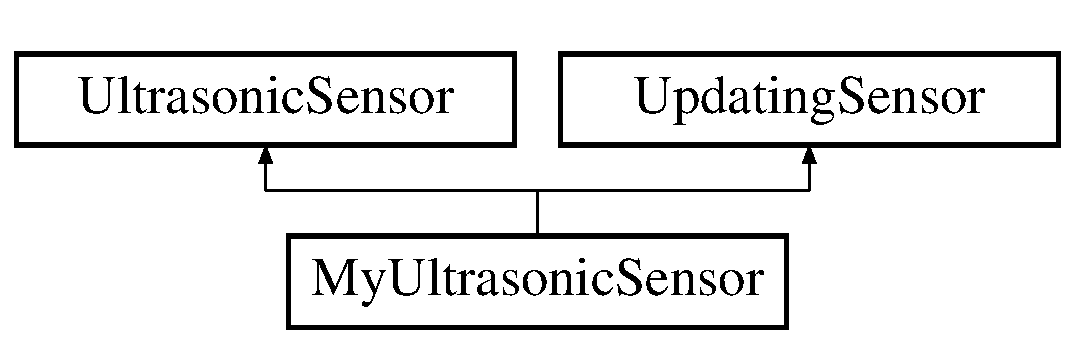
\includegraphics[height=2.000000cm]{class_my_ultrasonic_sensor}
\end{center}
\end{figure}
\subsection*{Public Member Functions}
\begin{DoxyCompactItemize}
\item 
\hyperlink{class_my_ultrasonic_sensor_afa87d140f6257f66ce04ddb2ee884d2a}{My\-Ultrasonic\-Sensor} (Sensor\-Port port)
\item 
void \hyperlink{class_my_ultrasonic_sensor_ac40ef007316dbc77871f8ca1cfd19b17}{add\-Listener} (\hyperlink{interface_sensor_listener}{Sensor\-Listener} lst)
\item 
void \hyperlink{class_my_ultrasonic_sensor_af7e1ac5d2e247d022f6a6d1fa387bf44}{update\-State} ()
\end{DoxyCompactItemize}


\subsection{Detailed Description}
\begin{DoxyAuthor}{Author}
Peter Markoti� 
\end{DoxyAuthor}
\begin{DoxyVersion}{Version}
2.\-0
\end{DoxyVersion}
Extended version of Ultrasonic\-Sensor. Passes new values from polling on to known listeners. 

\subsection{Constructor \& Destructor Documentation}
\hypertarget{class_my_ultrasonic_sensor_afa87d140f6257f66ce04ddb2ee884d2a}{\index{My\-Ultrasonic\-Sensor@{My\-Ultrasonic\-Sensor}!My\-Ultrasonic\-Sensor@{My\-Ultrasonic\-Sensor}}
\index{My\-Ultrasonic\-Sensor@{My\-Ultrasonic\-Sensor}!MyUltrasonicSensor@{My\-Ultrasonic\-Sensor}}
\subsubsection[{My\-Ultrasonic\-Sensor}]{\setlength{\rightskip}{0pt plus 5cm}My\-Ultrasonic\-Sensor.\-My\-Ultrasonic\-Sensor (
\begin{DoxyParamCaption}
\item[{Sensor\-Port}]{port}
\end{DoxyParamCaption}
)}}\label{class_my_ultrasonic_sensor_afa87d140f6257f66ce04ddb2ee884d2a}
Constructor. Defines port and instantiates array.


\begin{DoxyParams}{Parameters}
{\em port} & \\
\hline
\end{DoxyParams}


\subsection{Member Function Documentation}
\hypertarget{class_my_ultrasonic_sensor_ac40ef007316dbc77871f8ca1cfd19b17}{\index{My\-Ultrasonic\-Sensor@{My\-Ultrasonic\-Sensor}!add\-Listener@{add\-Listener}}
\index{add\-Listener@{add\-Listener}!MyUltrasonicSensor@{My\-Ultrasonic\-Sensor}}
\subsubsection[{add\-Listener}]{\setlength{\rightskip}{0pt plus 5cm}void My\-Ultrasonic\-Sensor.\-add\-Listener (
\begin{DoxyParamCaption}
\item[{{\bf Sensor\-Listener}}]{lst}
\end{DoxyParamCaption}
)}}\label{class_my_ultrasonic_sensor_ac40ef007316dbc77871f8ca1cfd19b17}
Add a \hyperlink{interface_sensor_listener}{Sensor\-Listener} to pass values on to.


\begin{DoxyParams}{Parameters}
{\em lst} & \\
\hline
\end{DoxyParams}
\hypertarget{class_my_ultrasonic_sensor_af7e1ac5d2e247d022f6a6d1fa387bf44}{\index{My\-Ultrasonic\-Sensor@{My\-Ultrasonic\-Sensor}!update\-State@{update\-State}}
\index{update\-State@{update\-State}!MyUltrasonicSensor@{My\-Ultrasonic\-Sensor}}
\subsubsection[{update\-State}]{\setlength{\rightskip}{0pt plus 5cm}void My\-Ultrasonic\-Sensor.\-update\-State (
\begin{DoxyParamCaption}
{}
\end{DoxyParamCaption}
)\hspace{0.3cm}{\ttfamily [virtual]}}}\label{class_my_ultrasonic_sensor_af7e1ac5d2e247d022f6a6d1fa387bf44}
Retrieves current sensor value, passes on to known Sensor\-Listeners if a change in value is detected.

\begin{DoxyReturn}{Returns}
void 
\end{DoxyReturn}


Implements \hyperlink{interface_updating_sensor}{Updating\-Sensor}.



The documentation for this class was generated from the following file\-:\begin{DoxyCompactItemize}
\item 
My\-Ultrasonic\-Sensor.\-java\end{DoxyCompactItemize}

\hypertarget{class_robot_controller}{\section{Robot\-Controller Class Reference}
\label{class_robot_controller}\index{Robot\-Controller@{Robot\-Controller}}
}
\subsection*{Public Member Functions}
\begin{DoxyCompactItemize}
\item 
\hyperlink{class_robot_controller_a8497b295f6b89c734357c9c0e1c2d4be}{Robot\-Controller} (\hyperlink{class_my_color_sensor}{My\-Color\-Sensor} right, \hyperlink{class_my_color_sensor}{My\-Color\-Sensor} left)
\item 
void \hyperlink{class_robot_controller_a2cb1bc61fba8750cacf883a8096d23ea}{process\-Ultrasonic} (float old\-Val, float new\-Val)
\item 
void \hyperlink{class_robot_controller_a56d8544ef554fa42ae14df568d836cc9}{process\-Right} (float old\-Val, float new\-Val)
\item 
void \hyperlink{class_robot_controller_ac923fcdf536fec9f25fc241af598696b}{process\-Left} (float old\-Val, float new\-Val)
\item 
void \hyperlink{class_robot_controller_a904bf3feb989cd825e92e618184b9d66}{check} ()
\item 
void \hyperlink{class_robot_controller_a81581974756705e965436ce7b9aff352}{drive\-Robot} ()
\end{DoxyCompactItemize}


\subsection{Detailed Description}
\begin{DoxyAuthor}{Author}
Kevin Nijmeijer, Michiel Tegelberg 
\end{DoxyAuthor}
\begin{DoxyVersion}{Version}
2.\-0 
\end{DoxyVersion}


\subsection{Constructor \& Destructor Documentation}
\hypertarget{class_robot_controller_a8497b295f6b89c734357c9c0e1c2d4be}{\index{Robot\-Controller@{Robot\-Controller}!Robot\-Controller@{Robot\-Controller}}
\index{Robot\-Controller@{Robot\-Controller}!RobotController@{Robot\-Controller}}
\subsubsection[{Robot\-Controller}]{\setlength{\rightskip}{0pt plus 5cm}Robot\-Controller.\-Robot\-Controller (
\begin{DoxyParamCaption}
\item[{{\bf My\-Color\-Sensor}}]{right, }
\item[{{\bf My\-Color\-Sensor}}]{left}
\end{DoxyParamCaption}
)}}\label{class_robot_controller_a8497b295f6b89c734357c9c0e1c2d4be}
Constructor for \hyperlink{class_robot_controller}{Robot\-Controller}

Makes an instance of \hyperlink{class_sensor_controller}{Sensor\-Controller} with the calibrated left and right Color\-Sensor. Makes an instance of \hyperlink{class_drive_controller}{Drive\-Controller} Sets the object\-Distance\-Limit to 20


\begin{DoxyParams}{Parameters}
{\em right} & the right calibrated \hyperlink{class_my_color_sensor}{My\-Color\-Sensor} from the \hyperlink{class_calibrate}{Calibrate} class. \\
\hline
{\em left} & the left calibrated \hyperlink{class_my_color_sensor}{My\-Color\-Sensor} from the \hyperlink{class_calibrate}{Calibrate} class. \\
\hline
\end{DoxyParams}


\subsection{Member Function Documentation}
\hypertarget{class_robot_controller_a904bf3feb989cd825e92e618184b9d66}{\index{Robot\-Controller@{Robot\-Controller}!check@{check}}
\index{check@{check}!RobotController@{Robot\-Controller}}
\subsubsection[{check}]{\setlength{\rightskip}{0pt plus 5cm}void Robot\-Controller.\-check (
\begin{DoxyParamCaption}
{}
\end{DoxyParamCaption}
)}}\label{class_robot_controller_a904bf3feb989cd825e92e618184b9d66}
Checks the current values for the Color\-Sensors versus the Threshold

\begin{DoxyReturn}{Returns}
void 
\end{DoxyReturn}
\hypertarget{class_robot_controller_a81581974756705e965436ce7b9aff352}{\index{Robot\-Controller@{Robot\-Controller}!drive\-Robot@{drive\-Robot}}
\index{drive\-Robot@{drive\-Robot}!RobotController@{Robot\-Controller}}
\subsubsection[{drive\-Robot}]{\setlength{\rightskip}{0pt plus 5cm}void Robot\-Controller.\-drive\-Robot (
\begin{DoxyParamCaption}
{}
\end{DoxyParamCaption}
)}}\label{class_robot_controller_a81581974756705e965436ce7b9aff352}
Sets the robot to drive forward at max\-Speed.

\begin{DoxyReturn}{Returns}
void 
\end{DoxyReturn}
\hypertarget{class_robot_controller_ac923fcdf536fec9f25fc241af598696b}{\index{Robot\-Controller@{Robot\-Controller}!process\-Left@{process\-Left}}
\index{process\-Left@{process\-Left}!RobotController@{Robot\-Controller}}
\subsubsection[{process\-Left}]{\setlength{\rightskip}{0pt plus 5cm}void Robot\-Controller.\-process\-Left (
\begin{DoxyParamCaption}
\item[{float}]{old\-Val, }
\item[{float}]{new\-Val}
\end{DoxyParamCaption}
)}}\label{class_robot_controller_ac923fcdf536fec9f25fc241af598696b}
Decides what to do with given Light valueof the left Color\-Sensor.


\begin{DoxyParams}{Parameters}
{\em old\-Val} & is not used \\
\hline
{\em new\-Val} & is the current value \\
\hline
\end{DoxyParams}
\begin{DoxyReturn}{Returns}
void 
\end{DoxyReturn}
\hypertarget{class_robot_controller_a56d8544ef554fa42ae14df568d836cc9}{\index{Robot\-Controller@{Robot\-Controller}!process\-Right@{process\-Right}}
\index{process\-Right@{process\-Right}!RobotController@{Robot\-Controller}}
\subsubsection[{process\-Right}]{\setlength{\rightskip}{0pt plus 5cm}void Robot\-Controller.\-process\-Right (
\begin{DoxyParamCaption}
\item[{float}]{old\-Val, }
\item[{float}]{new\-Val}
\end{DoxyParamCaption}
)}}\label{class_robot_controller_a56d8544ef554fa42ae14df568d836cc9}
Decides what to do with the given Light value of the right Color\-Sensor.


\begin{DoxyParams}{Parameters}
{\em old\-Val} & is not used \\
\hline
{\em new\-Val} & is the current value \\
\hline
\end{DoxyParams}
\begin{DoxyReturn}{Returns}
void 
\end{DoxyReturn}
\hypertarget{class_robot_controller_a2cb1bc61fba8750cacf883a8096d23ea}{\index{Robot\-Controller@{Robot\-Controller}!process\-Ultrasonic@{process\-Ultrasonic}}
\index{process\-Ultrasonic@{process\-Ultrasonic}!RobotController@{Robot\-Controller}}
\subsubsection[{process\-Ultrasonic}]{\setlength{\rightskip}{0pt plus 5cm}void Robot\-Controller.\-process\-Ultrasonic (
\begin{DoxyParamCaption}
\item[{float}]{old\-Val, }
\item[{float}]{new\-Val}
\end{DoxyParamCaption}
)}}\label{class_robot_controller_a2cb1bc61fba8750cacf883a8096d23ea}
Decides what to do with the given Ultrasonic value


\begin{DoxyParams}{Parameters}
{\em old\-Val} & the last updated value for the Ultrasonic Value \\
\hline
{\em new\-Val} & the current value for Ultrasonic \\
\hline
\end{DoxyParams}
\begin{DoxyReturn}{Returns}
void 
\end{DoxyReturn}


The documentation for this class was generated from the following file\-:\begin{DoxyCompactItemize}
\item 
Robot\-Controller.\-java\end{DoxyCompactItemize}

\hypertarget{class_sensor_controller}{\section{Sensor\-Controller Class Reference}
\label{class_sensor_controller}\index{Sensor\-Controller@{Sensor\-Controller}}
}
Inheritance diagram for Sensor\-Controller\-:\begin{figure}[H]
\begin{center}
\leavevmode
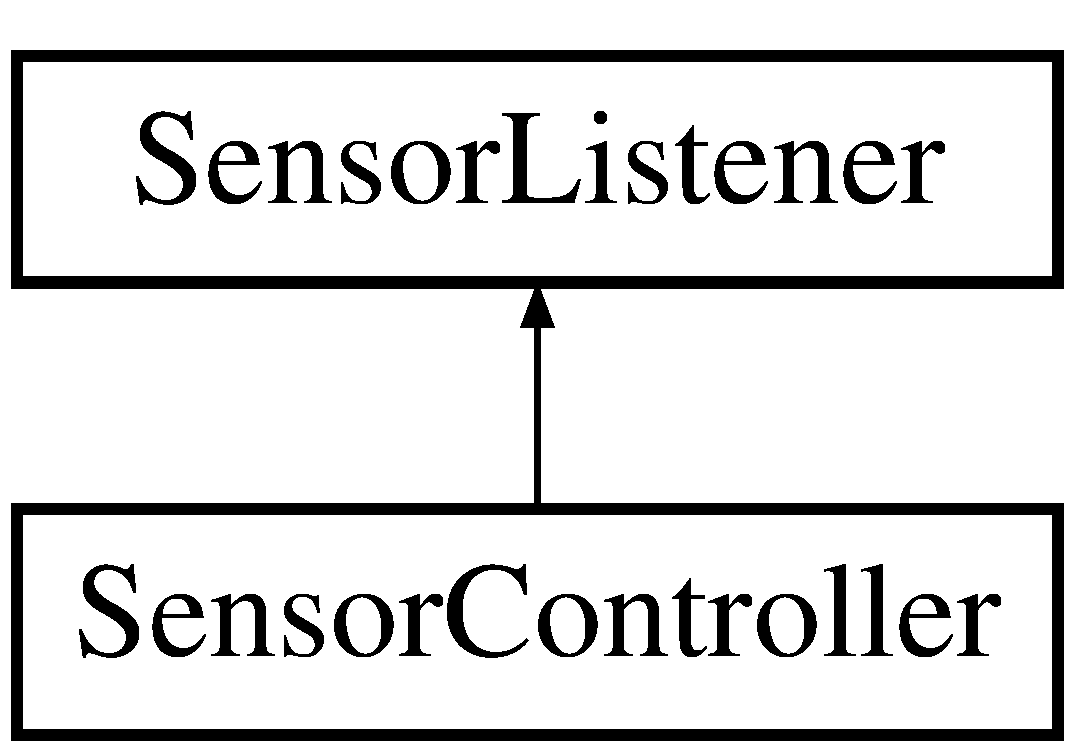
\includegraphics[height=2.000000cm]{class_sensor_controller}
\end{center}
\end{figure}
\subsection*{Public Member Functions}
\begin{DoxyCompactItemize}
\item 
\hyperlink{class_sensor_controller_adbd82a25c1500ca6d4f877c03f609c90}{Sensor\-Controller} (\hyperlink{class_robot_controller}{Robot\-Controller} rc, \hyperlink{class_my_color_sensor}{My\-Color\-Sensor} right, \hyperlink{class_my_color_sensor}{My\-Color\-Sensor} left)
\item 
void \hyperlink{class_sensor_controller_a7cac7725250f0d1b49ef1d09d6c4071d}{state\-Changed} (\hyperlink{interface_updating_sensor}{Updating\-Sensor} s, float old\-Val, float new\-Val)
\end{DoxyCompactItemize}


\subsection{Detailed Description}
\begin{DoxyAuthor}{Author}
Peter Markoti�, Michiel Tegelberg 
\end{DoxyAuthor}
\begin{DoxyVersion}{Version}
2.\-0
\end{DoxyVersion}
\hyperlink{class_sensor_controller}{Sensor\-Controller} is the receiver of all changed states and values of the sensors. After receiving, it has the ability to decide what is to be done with those values, calling actions from Motor\-Controller 

\subsection{Constructor \& Destructor Documentation}
\hypertarget{class_sensor_controller_adbd82a25c1500ca6d4f877c03f609c90}{\index{Sensor\-Controller@{Sensor\-Controller}!Sensor\-Controller@{Sensor\-Controller}}
\index{Sensor\-Controller@{Sensor\-Controller}!SensorController@{Sensor\-Controller}}
\subsubsection[{Sensor\-Controller}]{\setlength{\rightskip}{0pt plus 5cm}Sensor\-Controller.\-Sensor\-Controller (
\begin{DoxyParamCaption}
\item[{{\bf Robot\-Controller}}]{rc, }
\item[{{\bf My\-Color\-Sensor}}]{right, }
\item[{{\bf My\-Color\-Sensor}}]{left}
\end{DoxyParamCaption}
)}}\label{class_sensor_controller_adbd82a25c1500ca6d4f877c03f609c90}
Constructor for \hyperlink{class_sensor_controller}{Sensor\-Controller} Sets the \hyperlink{class_robot_controller}{Robot\-Controller} Instance and adds the Sensors to the \hyperlink{class_sensor_handler}{Sensor\-Handler}.


\begin{DoxyParams}{Parameters}
{\em rc} & The instance of \hyperlink{class_robot_controller}{Robot\-Controller} \\
\hline
{\em right} & The right \hyperlink{class_my_color_sensor}{My\-Color\-Sensor} \\
\hline
{\em left} & The left \hyperlink{class_my_color_sensor}{My\-Color\-Sensor} \\
\hline
\end{DoxyParams}


\subsection{Member Function Documentation}
\hypertarget{class_sensor_controller_a7cac7725250f0d1b49ef1d09d6c4071d}{\index{Sensor\-Controller@{Sensor\-Controller}!state\-Changed@{state\-Changed}}
\index{state\-Changed@{state\-Changed}!SensorController@{Sensor\-Controller}}
\subsubsection[{state\-Changed}]{\setlength{\rightskip}{0pt plus 5cm}void Sensor\-Controller.\-state\-Changed (
\begin{DoxyParamCaption}
\item[{{\bf Updating\-Sensor}}]{s, }
\item[{float}]{old\-Val, }
\item[{float}]{new\-Val}
\end{DoxyParamCaption}
)\hspace{0.3cm}{\ttfamily [virtual]}}}\label{class_sensor_controller_a7cac7725250f0d1b49ef1d09d6c4071d}
Inherited from interface, receiver values from polled sensors, then sends these through to individual methods for each type of sensor.


\begin{DoxyParams}{Parameters}
{\em s} & \\
\hline
{\em old\-Val} & \\
\hline
{\em new\-Val} & \\
\hline
\end{DoxyParams}
\begin{DoxyReturn}{Returns}
void 
\end{DoxyReturn}


Implements \hyperlink{interface_sensor_listener}{Sensor\-Listener}.



The documentation for this class was generated from the following file\-:\begin{DoxyCompactItemize}
\item 
Sensor\-Controller.\-java\end{DoxyCompactItemize}

\hypertarget{class_sensor_handler}{\section{Sensor\-Handler Class Reference}
\label{class_sensor_handler}\index{Sensor\-Handler@{Sensor\-Handler}}
}
Inheritance diagram for Sensor\-Handler\-:\begin{figure}[H]
\begin{center}
\leavevmode
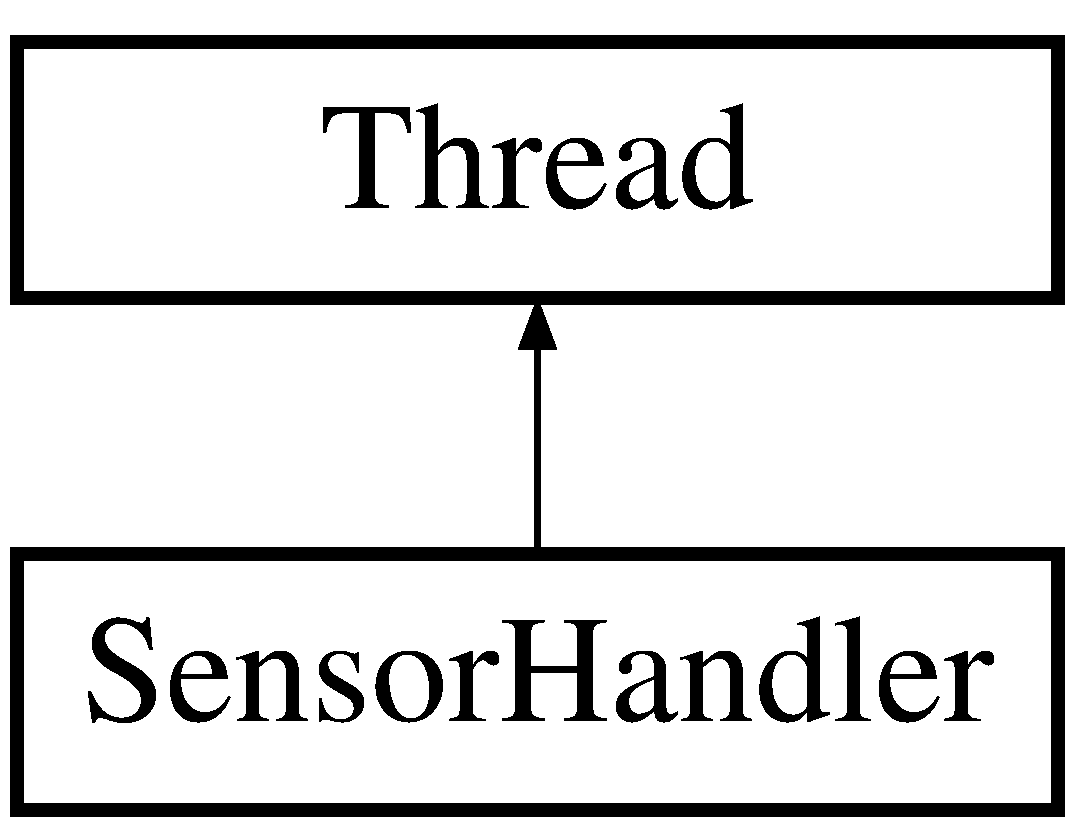
\includegraphics[height=2.000000cm]{class_sensor_handler}
\end{center}
\end{figure}
\subsection*{Public Member Functions}
\begin{DoxyCompactItemize}
\item 
void \hyperlink{class_sensor_handler_abd37546cd6e5ab5a88f81f07fdc679ef}{add\-Sensor} (\hyperlink{interface_updating_sensor}{Updating\-Sensor} us)
\item 
void \hyperlink{class_sensor_handler_afc263497e055f62dbd9e650aaa10611c}{run} ()
\end{DoxyCompactItemize}
\subsection*{Static Public Member Functions}
\begin{DoxyCompactItemize}
\item 
static \hyperlink{class_sensor_handler}{Sensor\-Handler} \hyperlink{class_sensor_handler_a67a5f768ddab8ef68ea49c3d82ca8fcf}{get\-Instance} ()
\end{DoxyCompactItemize}


\subsection{Detailed Description}
\begin{DoxyAuthor}{Author}
Peter Markoti� 
\end{DoxyAuthor}
\begin{DoxyVersion}{Version}
2.\-0
\end{DoxyVersion}
Holds an array of Updating\-Sensors and polls each once every given period of time. 

\subsection{Member Function Documentation}
\hypertarget{class_sensor_handler_abd37546cd6e5ab5a88f81f07fdc679ef}{\index{Sensor\-Handler@{Sensor\-Handler}!add\-Sensor@{add\-Sensor}}
\index{add\-Sensor@{add\-Sensor}!SensorHandler@{Sensor\-Handler}}
\subsubsection[{add\-Sensor}]{\setlength{\rightskip}{0pt plus 5cm}void Sensor\-Handler.\-add\-Sensor (
\begin{DoxyParamCaption}
\item[{{\bf Updating\-Sensor}}]{us}
\end{DoxyParamCaption}
)}}\label{class_sensor_handler_abd37546cd6e5ab5a88f81f07fdc679ef}
Adds an \hyperlink{interface_updating_sensor}{Updating\-Sensor} to array for polling


\begin{DoxyParams}{Parameters}
{\em us} & \\
\hline
\end{DoxyParams}
\begin{DoxyReturn}{Returns}
void 
\end{DoxyReturn}
\hypertarget{class_sensor_handler_a67a5f768ddab8ef68ea49c3d82ca8fcf}{\index{Sensor\-Handler@{Sensor\-Handler}!get\-Instance@{get\-Instance}}
\index{get\-Instance@{get\-Instance}!SensorHandler@{Sensor\-Handler}}
\subsubsection[{get\-Instance}]{\setlength{\rightskip}{0pt plus 5cm}static {\bf Sensor\-Handler} Sensor\-Handler.\-get\-Instance (
\begin{DoxyParamCaption}
{}
\end{DoxyParamCaption}
)\hspace{0.3cm}{\ttfamily [static]}}}\label{class_sensor_handler_a67a5f768ddab8ef68ea49c3d82ca8fcf}
Retrieves a reference to the \hyperlink{class_sensor_handler}{Sensor\-Handler}.

\begin{DoxyReturn}{Returns}
\hyperlink{class_sensor_handler}{Sensor\-Handler} 
\end{DoxyReturn}
\hypertarget{class_sensor_handler_afc263497e055f62dbd9e650aaa10611c}{\index{Sensor\-Handler@{Sensor\-Handler}!run@{run}}
\index{run@{run}!SensorHandler@{Sensor\-Handler}}
\subsubsection[{run}]{\setlength{\rightskip}{0pt plus 5cm}void Sensor\-Handler.\-run (
\begin{DoxyParamCaption}
{}
\end{DoxyParamCaption}
)}}\label{class_sensor_handler_afc263497e055f62dbd9e650aaa10611c}
Starts Thread for \hyperlink{class_sensor_handler}{Sensor\-Handler}

\begin{DoxyReturn}{Returns}
void 
\end{DoxyReturn}


The documentation for this class was generated from the following file\-:\begin{DoxyCompactItemize}
\item 
Sensor\-Handler.\-java\end{DoxyCompactItemize}

\hypertarget{interface_sensor_listener}{\section{Sensor\-Listener Interface Reference}
\label{interface_sensor_listener}\index{Sensor\-Listener@{Sensor\-Listener}}
}
Inheritance diagram for Sensor\-Listener\-:\begin{figure}[H]
\begin{center}
\leavevmode
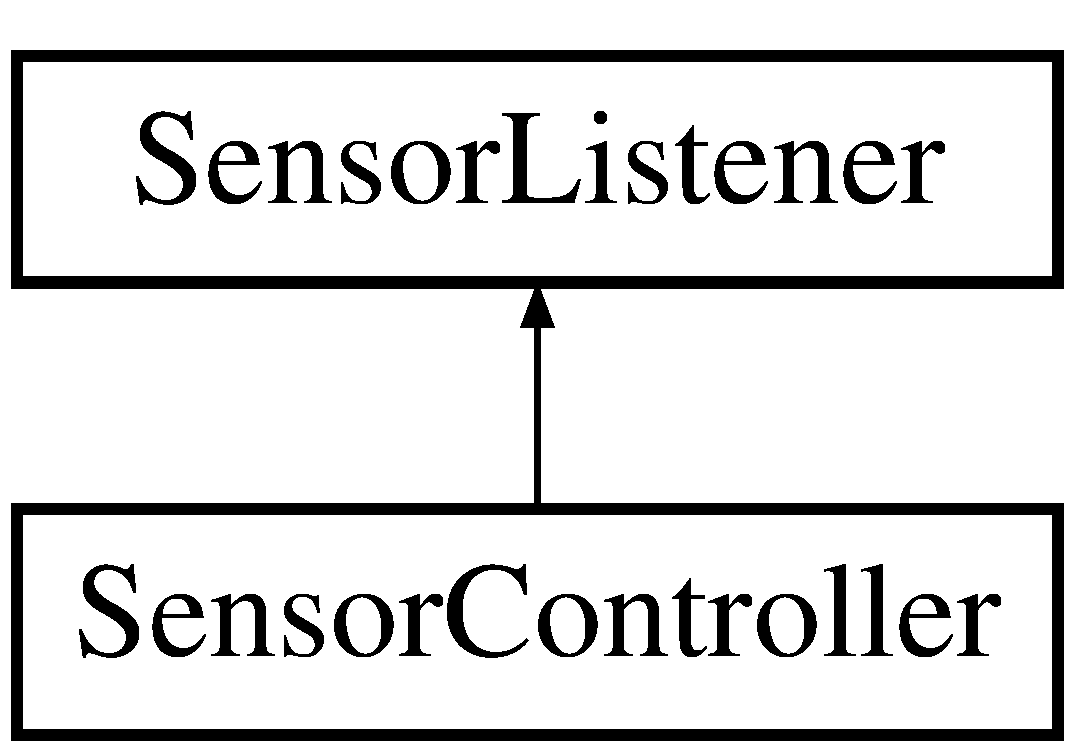
\includegraphics[height=2.000000cm]{interface_sensor_listener}
\end{center}
\end{figure}
\subsection*{Public Member Functions}
\begin{DoxyCompactItemize}
\item 
\hypertarget{interface_sensor_listener_a25fd6351f26a35199c2af82b528e3afa}{abstract void {\bfseries state\-Changed} (\hyperlink{interface_updating_sensor}{Updating\-Sensor} s, float old\-Val, float new\-Val)}\label{interface_sensor_listener_a25fd6351f26a35199c2af82b528e3afa}

\end{DoxyCompactItemize}


\subsection{Detailed Description}
\begin{DoxyAuthor}{Author}
Peter Markoti� 
\end{DoxyAuthor}
\begin{DoxyVersion}{Version}
1.\-0
\end{DoxyVersion}
Defines the state\-Changed method for Sensor\-Listeners 

The documentation for this interface was generated from the following file\-:\begin{DoxyCompactItemize}
\item 
Sensor\-Listener.\-java\end{DoxyCompactItemize}

\hypertarget{interface_updating_sensor}{\section{Updating\-Sensor Interface Reference}
\label{interface_updating_sensor}\index{Updating\-Sensor@{Updating\-Sensor}}
}
Inheritance diagram for Updating\-Sensor\-:\begin{figure}[H]
\begin{center}
\leavevmode
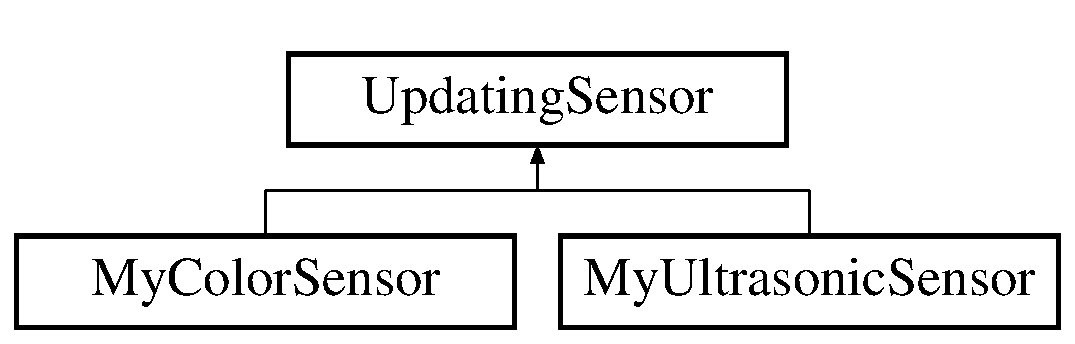
\includegraphics[height=2.000000cm]{interface_updating_sensor}
\end{center}
\end{figure}
\subsection*{Public Member Functions}
\begin{DoxyCompactItemize}
\item 
\hypertarget{interface_updating_sensor_abf0400bc7444bfd96ed70a9be75dd34a}{abstract void {\bfseries update\-State} ()}\label{interface_updating_sensor_abf0400bc7444bfd96ed70a9be75dd34a}

\end{DoxyCompactItemize}


\subsection{Detailed Description}
\begin{DoxyAuthor}{Author}
Peter Markoti� 
\end{DoxyAuthor}
\begin{DoxyVersion}{Version}
1.\-0
\end{DoxyVersion}
Defines update\-State() method for Updating\-Sensors. 

The documentation for this interface was generated from the following file\-:\begin{DoxyCompactItemize}
\item 
Updating\-Sensor.\-java\end{DoxyCompactItemize}

%--- End generated contents ---

% Index
\newpage
\phantomsection
\addcontentsline{toc}{part}{Index}
\printindex

\end{document}
